\documentclass[11pt]{article}
\usepackage{textcomp,geometry,graphicx,verbatim}
\usepackage{fancyhdr}
\usepackage{amsmath,amssymb,enumerate}
\pagestyle{fancy}
\def\Name{Manohar Jois}
\def\Homework{2} % Homework number - make sure to change for every homework!
\def\Session{Fall 2014}

% Extra commands
\let\origleft\left
\let\origright\right
\renewcommand{\left}{\mathopen{}\mathclose\bgroup\origleft}
\renewcommand{\right}{\aftergroup\egroup\origright}
\newcommand{\N}{\mathbb{N}}
\newcommand{\Z}{\mathbb{Z}}
\newcommand{\R}{\mathbb{R}}
\newcommand{\Q}{\mathbb{Q}}
\newcommand{\C}{\mathbb{C}}
\newcommand{\p}[1]{\left(#1\right)}
\renewcommand{\gcd}[1]{\text{gcd}\p{#1}}
\renewcommand{\deg}[1]{\text{deg}\p{#1}}
\renewcommand{\log}[1]{\text{log}\p{#1}}
\renewcommand{\ln}[1]{\text{ln}\p{#1}}
\newcommand{\logb}[2]{\text{log}_{#1}\p{#2}}
\newcommand{\BigOh}[1]{O\p{#1}}
\newcommand{\BigOmega}[1]{\Omega\p{#1}}
\newcommand{\BigTheta}[1]{\Theta\p{#1}}

\title{CS164\ \Session\  --- Answers to Homework \Homework}
\author{\Name}
\lhead{CS164\ \Session\  Homework \Homework\ Problem \theproblemnumber,\ \Name}

\begin{document}
\maketitle
\newcounter{problemnumber}
\setcounter{problemnumber}{0}

\section*{Exercise 1}
\stepcounter{problemnumber}
\begin{enumerate}[(a)]
\item The code will log \texttt{initial message} on the first line and \texttt{meet me by the docks at midnight} on the second. The function \texttt{getMessage} returns the variable \texttt{message} bound in the local scope of the outer anonymous function, and the setter binds the same variable to its argument.
\item Environment diagram:\\
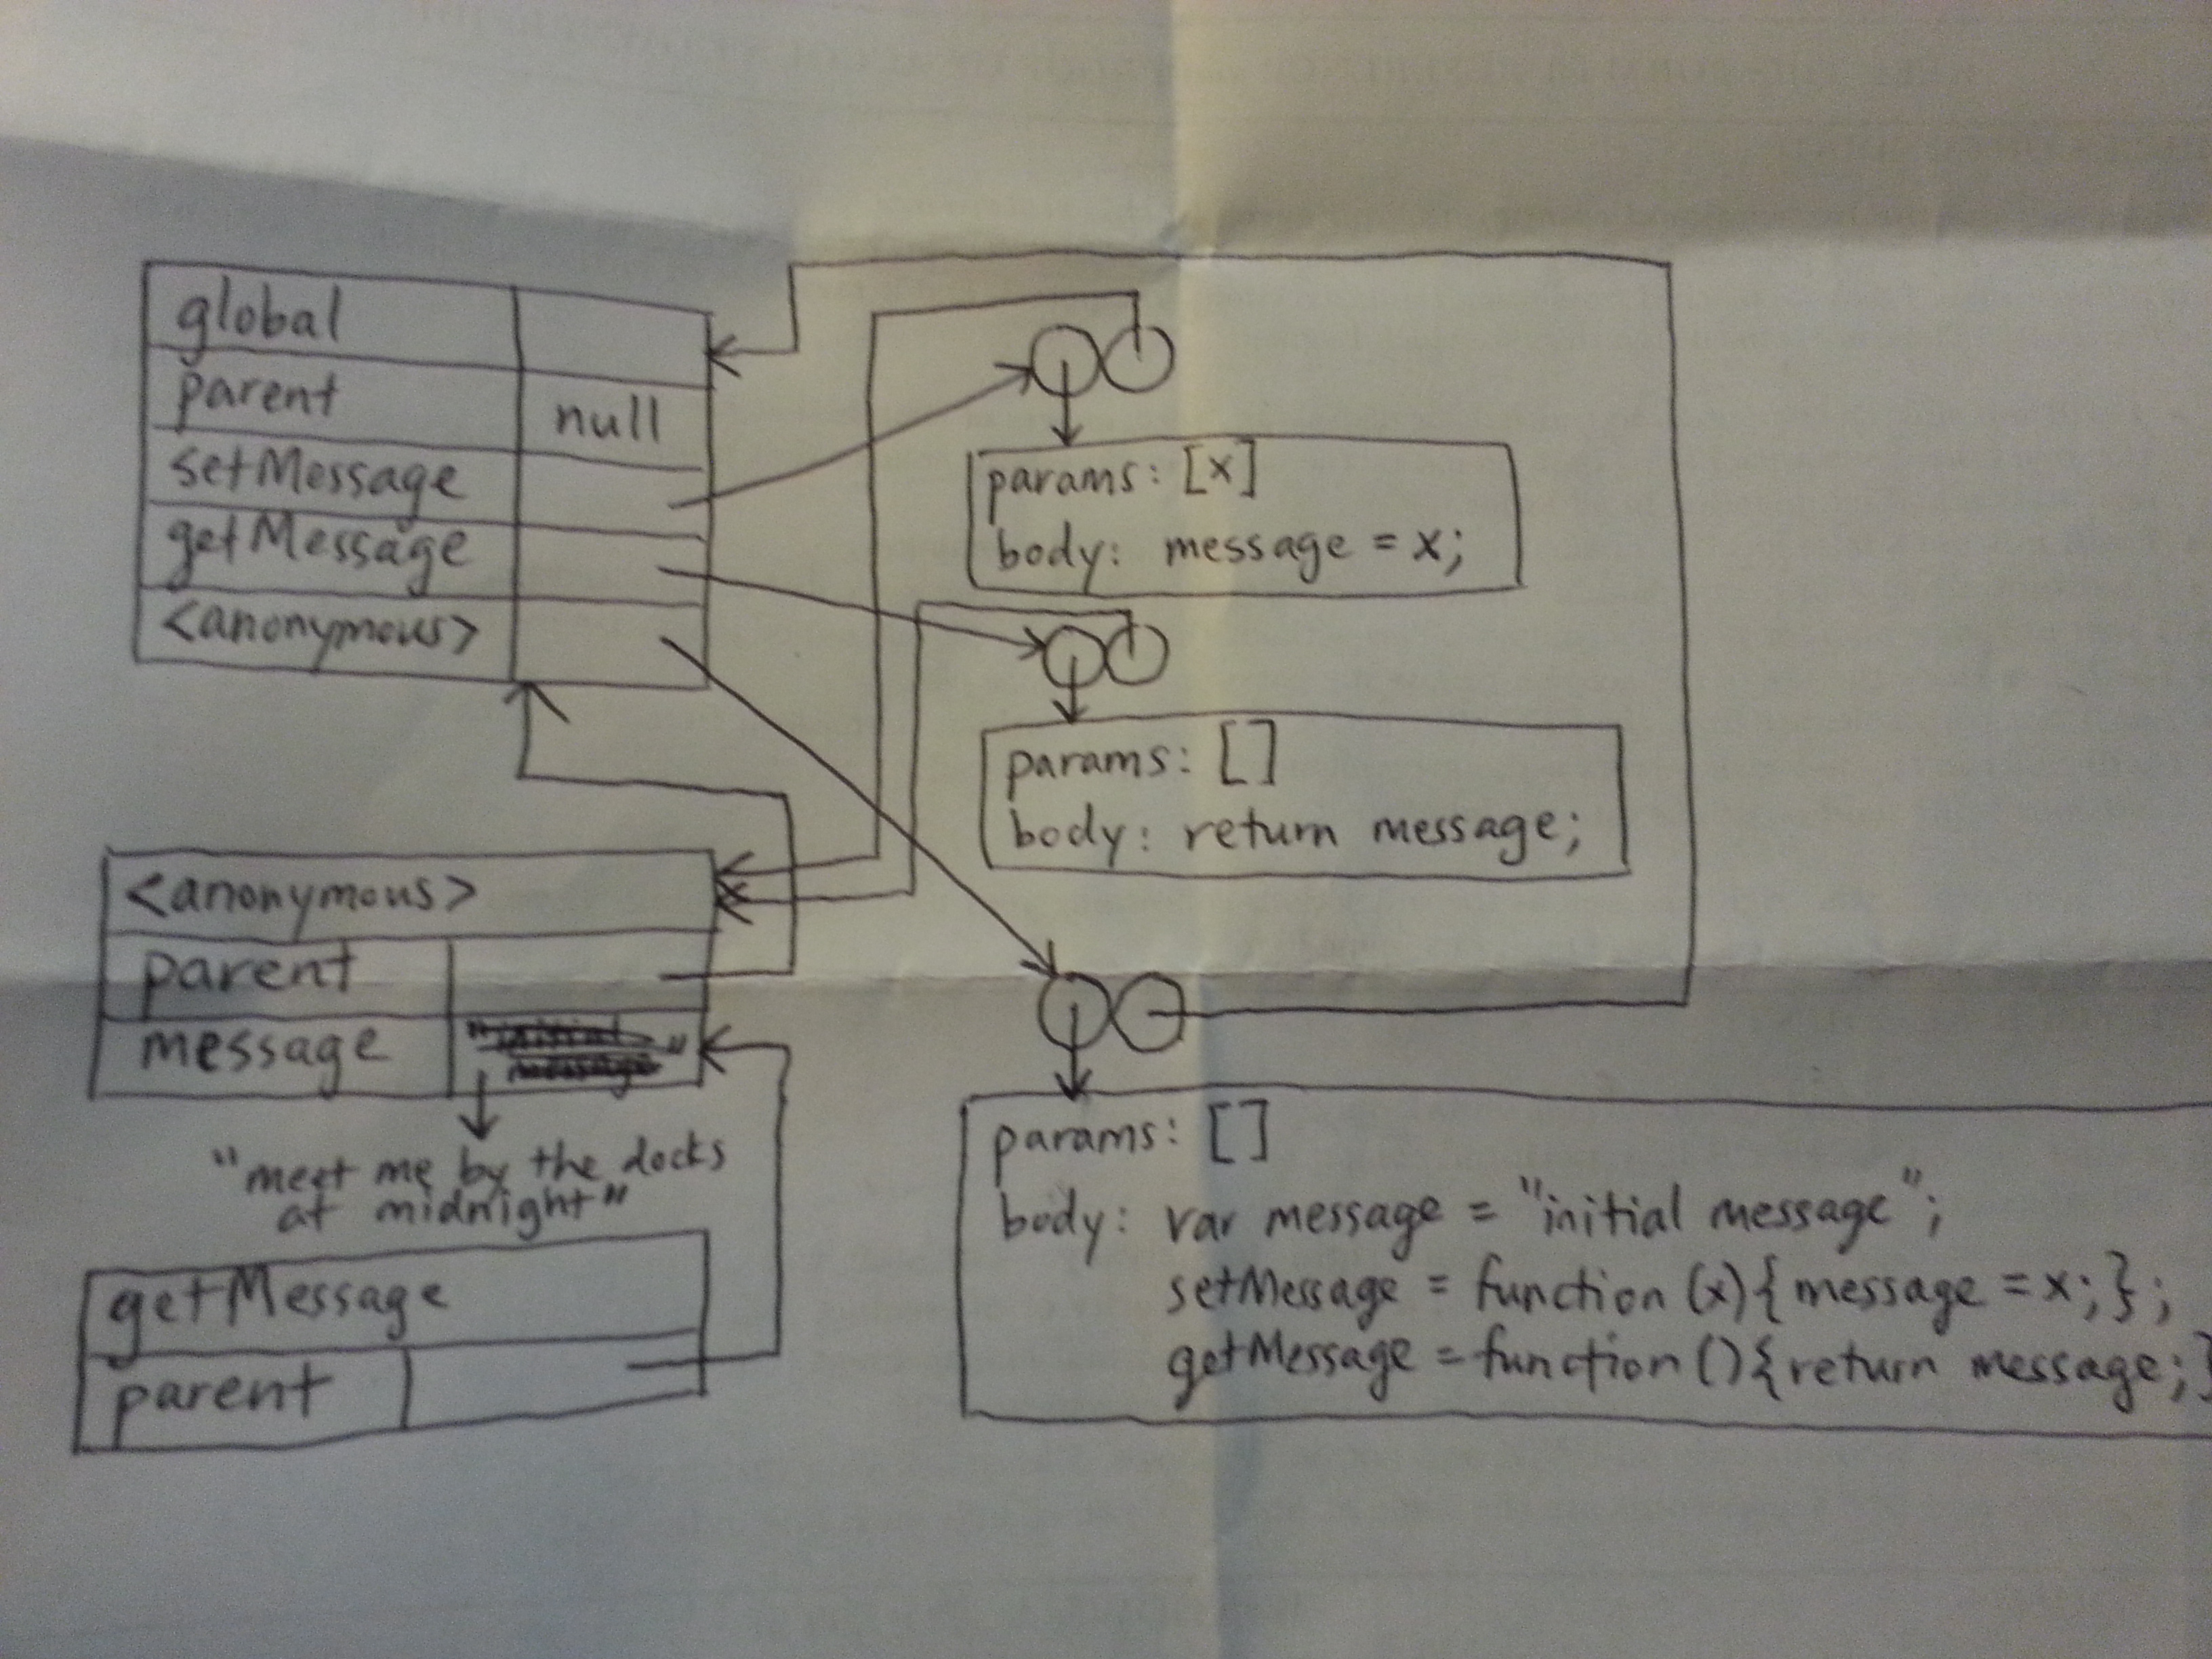
\includegraphics[scale=0.125]{env}
\item The code will log \texttt{This string is even cooler.} on the first line and \texttt{This string is the coolest!} on the second. The first output comes from logging the value of local variable \texttt{a} inside the function \texttt{cooler}. Meanwhile, calling \texttt{coolest} binds the global variable \texttt{a} because it's not defined locally with \texttt{var}.
\item With dynamic scoping, the code would log \texttt{This string is the coolest!} twice. Calling \texttt{coolest} before logging \texttt{a} for the first time pushes that string into the stack of bindings for \texttt{a}, and it doesn't change throughout the rest of the program.
\end{enumerate}


\newpage
\section*{Exercise 2}
\stepcounter{problemnumber}
\begin{enumerate}[(a)]
\item I would expect the code to print "c" then "a" then "l" in that order, each on its own line. Each new anonymous function created should be part of a closure that holds the value of \texttt{index} at the time it was created, and so the three lambdas should return the three elements of the array.
\item The semantics of the for-loop seem to suggest that at each iteration, \texttt{index} is bound to the next element of the array, not the index of that element. This would produce three \texttt{undefined} lines because of array accesses like \texttt{array["c"]}.
\item The output was three "l" characters, each on its own line. This is probably because the \texttt{index} variable in the body of the anonymous functions references the \texttt{index} variable in the scope of the for-loop, and it is last bound to the value 2 because that's the last index of the array. Calling the three lambdas after the for-loop executes means they all access \texttt{array[2]}.
\item Equivalent code in Python: \begin{verbatim}
array = ["c","a","l"]
lambdas = []

for index in array:
    lambdas.append(lambda: array[index])

print(lambdas[0]())
print(lambdas[1]())
print(lambdas[2]())
\end{verbatim}
Output:
\begin{verbatim}
mj@mjubuntu:~/Documents/cs164/hw2$ python e2d.py
Traceback (most recent call last):
  File "e2d.py", line 7, in <module>
    print(lambdas[0]())
  File "e2d.py", line 5, in <lambda>
    lambdas.append(lambda: array[index])
TypeError: list indices must be integers, not str
mj@mjubuntu:~/Documents/cs164/hw2$
\end{verbatim}
Python exhibits the semantics suggested in 2(b), and throws an error upon an improper array access.
\end{enumerate}


\newpage
\section*{Exercise 3}
\stepcounter{problemnumber}
\begin{enumerate}[(a)]
\item \begin{verbatim}
"for" : "def %u1 = %iterator(); \
         while (%u1 !== null) { \
            def %name = %u1; \
            (lambda(){%body})() \
            %u1 = %iterator(); \
         }"
\end{verbatim}
\item \begin{verbatim}
"for" : "def %u1 = %iterator(); \
         while (%u1 !== null) { \
            (lambda(){ \
                def %name = %u1; \
                (lambda(){%body})() \
                %u1 = %iterator(); \
            })() \
         }"
\end{verbatim}
\end{enumerate}

\end{document}